\documentclass{article}
\pdfpagewidth=8.5in
\pdfpageheight=11in
\usepackage{ijcai19}
% The file ijcai18.sty is the style file for IJCAI-18 (same as ijcai08.sty).

% Use the postscript times font!
\usepackage{times}
\usepackage{soul}
\usepackage{url}
\usepackage[hidelinks]{hyperref}

\usepackage[utf8]{inputenc}
\usepackage[english]{babel}
\usepackage[small]{caption}

%%%%%%
\newtheorem{theorem}{Theorem}

% Math notation
\RequirePackage[group-separator={,}]{siunitx}
\newcommand{\na}{$\mathrm{N.A.}$}
\newcommand{\minus}{\scalebox{0.7}[1.0]{$-$}}
\newcommand{\expn}[1]{\!\!\times\!\!10^{\minus#1}}
\newcommand{\pval}[2]{$p\textrm{-value} = #1\expn{#2}$}
\newcommand{\set}[1]{\{{}#1\}}
\newcommand{\A}[1]{\mathcal{A}_{#1}}
\newcommand{\N}[1]{n_{#1}(j)}



%%%%%%
\usepackage{float}
\usepackage{listings}
\usepackage{caption}
\usepackage{graphicx}
\usepackage{subcaption}
\usepackage{colortbl}
\usepackage{amsmath}
%\usepackage{amsthm} 
\usepackage{mathpartir}
\usepackage{fancyvrb}\fvset{fontsize=\small}
\usepackage{xspace}
\usepackage{xcolor}
\usepackage{balance}
\usepackage{wrapfig}
\usepackage{multirow}
\usepackage{pifont}
\usepackage{amssymb}
%%%%%%%%%%%%%%%%%%% this can reduce space quite a lot
\usepackage{soul}
\usepackage{microtype}
\usepackage[T1]{fontenc}
\usepackage{dsfont}
%%%%%%%%%%%%%%%%%%% this can reduce space quite a lot
\usepackage{relsize}
\usepackage{tikz}
\usepackage{longtable}
\usepackage{booktabs}
\usepackage{marvosym} 
\usepackage{framed}
\usepackage{mdwlist}
\usepackage{tabularx}
\usepackage{wrapfig}

\usepackage{array}
\usepackage{mathtools}
\usepackage{url}
\usepackage{color}

%% Colors
\definecolor{bgBlock}{rgb}{0.22,0.15,0.49}
\definecolor{bgBlockAlert}{rgb}{0.99,0.84,0.31}
\definecolor{fgBlockAlert}{rgb}{0.22,0.15,0.49}
\definecolor{fgBlock}{rgb}{0.99,0.84,0.31}
\definecolor{darkred}{rgb}{0.5,0,0}
\definecolor{darkgreen}{rgb}{0,0.5,0}
\definecolor{darkblue}{rgb}{0,0,0.5}
\definecolor{Gray}{gray}{0.9}

%%%%%%%%%% added by sofia
\usepackage{algpseudocode}
\usepackage{algorithm}
\usepackage{enumitem}


\usepackage{bm}
\usepackage{cleveref}
\usepackage{textcomp}
\usepackage{pdfpages}
\usepackage{chngpage}


%\usepackage[hyphenbreaks]{breakurl}


%%%%%%%%%%

\usepackage[most]{tcolorbox}
\newtcolorbox{myframe}[1][]{
	enhanced,
	arc=0pt,
	outer arc=0pt,
	colback=white,
	boxrule=0.5pt,
	boxsep=1pt,left=3pt,right=3pt,top=5pt,bottom=5pt,
	fontupper=\small,
	size=small
	#1
}

%%%%%%%%%%
% appendix 
\usepackage[toc,page]{appendix}
\usepackage{makecell}


%%%%% Theorem -> Claim

\newtheorem{thm}{Theorem} % the main one
\newtheorem{lemma}[thm]{Lemma}

\newcommand{\thistheoremname}{}
\newtheorem{genericthm}[thm]{\thistheoremname}
\newenvironment{namedthm}[1]
  {\renewcommand{\thistheoremname}{#1}
   \begin{genericthm}}
  {\end{genericthm}}





\newcommand{\Fix}[1]{\textbf{[[}{\color{red} #1}\textbf{]]}}
\newcommand{\Anonim}[2]{#1}
\newcommand{\ie}{i.e.}
\newcommand{\eg}{e.g.}
\newcommand{\cf}{cf.}
\newcommand{\etal}{et al.}
\newcommand{\comments}[1]{}
\newcommand{\varex}{\textsc{Varex}}
\newcommand{\tsig}{OUR}
\newcommand{\tnamepar}[1]{\tname{}\texttt{[#1]}}
\newcommand{\CodeIn}[1]{{\small\texttt{#1}}}
\newcommand{\pw}{\textsc{pw}}
\newcommand{\pwopt}{\textsc{pw-opt}}
\newcommand{\dd}{\CodeIn{DD}}
\newcommand{\acrAbrev}{APR}
\newcommand{\RQ}{RQ}
\newcommand{\morpho}{\emph{morpho}}
\newcommand{\lithium}{\emph{lithium-slicer}}
\newcommand{\success}{\leavevmode\color[HTML]{009901}}

\definecolor{bs}{rgb}{0.59, 0.0, 0.09}
\definecolor{d}{HTML}{800000}

\newcommand{\BS}[1]{\textbf{[BS:[}{\color{bs} #1}\textbf{]]}}
\newcommand{\Mar}[1]{\textbf{[Marcelo:[}{\color{orange} #1}\textbf{]]}}
\newcommand{\Sof}[1]{\textbf{[Sofia:[}{\color{cyan} #1}\textbf{]]}}
\newcommand{\oururl}{\Fix{url here}}
\newcommand{\tname}{\Fix{Critical Slicing Revisited}}

\newcommand{\numPrograms}{six}
\newcommand{\numFaults}{395}
\newcommand{\topk}{top-$k$}

\newcommand{\sfl}{SFL}
\newcommand{\CS}{CS}
\newcommand{\cs}{CS}
\newcommand{\ds}{DS}
\newcommand{\dfj}{Defects4J}
\newcommand{\orbs}{ORBS}
\newcommand{\comb}{\sfl{}+\ds{}}
\newcommand{\apr}{APR}

%% subject names as in https://github.com/rjust/defects4j
\newcommand{\chart}{JFreechart}
\newcommand{\closure}{Closure compiler}
\newcommand{\lang}{Apache commons-lang}
\newcommand{\cmath}{Apache commons-math}
\newcommand{\mockito}{Mockito}
\newcommand{\jtime}{Joda-Time}

\newcommand{\cmark}{\ding{51}}%
\newcommand{\xmark}{\ding{55}}%


% the following package is optional:
\usepackage{latexsym}

\title{Demystifying the Combination of Dynamic Slicing and \\ Spectrum-based Fault
Localization}

% Single author syntax
\author{
    Submission 6364
}
\iffalse
\author{
First Author$^1$
\and
Second Author$^2$\and
Third Author$^{2,3}$\And
Fourth Author$^4$
\affiliations
$^1$First Affiliation\\
$^2$Second Affiliation\\
$^3$Third Affiliation\\
$^4$Fourth Affiliation
\emails
\{first, second\}@example.com,
third@other.example.com,
fourth@example.com
}
\fi

\hypersetup{draft}
\begin{document}

\maketitle

\begin{abstract}
Several approaches have been proposed in the literature to reduce
debugging costs through automated software fault diagnosis.  Dynamic
Slicing (\ds{}) and Spectrum-based Fault Localization (\sfl{}) are
popular fault diagnosis techniques and normally seen as complementary.
This paper reports on a comprehensive study\comments{--using
  \numFaults{} documented software faults from a credible dataset--}
to evaluate the effects of combining \ds{} with \sfl{}. We suspect
that several highly suspicious components---often involved in failing,
but seldom in passing test runs---may be unrelated to the bug. With
the aforementioned combination, such components could be located and
their suspiciousness reduced.  This study also discusses the practical
impact of the \ds{} key limitation---the risk of missing faulty
statements. Results indicate that \ds{} misses faulty statements in
 9\%\comments{(23 misses)} of the \numFaults{} cases and that
the \ds{}-\sfl{} combination, coined as Tandem-SL, improves on average
the diagnostic accuracy by \avgImprov\ in 51\% of the cases. To sum,
we found that the \ds{}-\sfl{} combination was practical and effective
and encourage new \sfl{} techniques to be evaluated against that
optimization.
\end{abstract}


\section{Introduction}

%% provide context (debugging + fault localization)
Software debugging is important and challenging. The task of locating
the faulty code (\ie{}, fault localization) is particularly
challenging. As such, countless automated techniques have been
proposed in the past to reduce the cost of fault
localization~\cite{7390282}. Model-based software diagnosis
(MBSD)~\cite{REITER198757,DEKLEER200325} and Spectrum-Based Fault
Localization (\sfl{})~\cite{DBLP:journals/stvr/HarroldRSWY00} are two
popular techniques that leverage different principles to automate
fault isolation~\cite{DBLP:conf/sac/AbreuGZG08}.  At a high-level,
MBSD
techniques~\cite{wotawa2002model,Mayer:2008:EMM:1642931.1642950,mayer2008prioritising,Perez:2018:LQR:3304889.3304927,Ko:2008:DRA:1368088.1368130}
attempt to eliminate non-suspicious components whereas \sfl{}
techniques attempt to rank suspicious components with the goal of
reducing fault diagnosis cost.

%% detail context (DS + SFL)
Dynamic Slicing (DS)~\cite{Agrawal:1990:DPS:93542.93576} is an
instance of MBSD that has attracted huge attention in research over
the last decades~\cite{Silva:2012:VPS:2187671.2187674}. The technique
traces back the statements in the code that influence a given point of
interest, such as the evaluation of a failing assertion.  Similarly to
\ds{}, \sfl{}~\cite{DBLP:journals/stvr/HarroldRSWY00} received
tremendous attention in research over the years~\cite{7390282}.  It
computes suspiciousness values associated with program components
(e.g., statements) based on coverage information gathered during the
execution of test cases.  More precisely, \sfl{} uses coverage
information of passing and failing test cases to identify likely
faulty statements and produces on output a list of program components
ranked in decreasing order of suspiciousness.

%% \ds{} and \sfl{} are complementary~\cite{DBLP:conf/sac/AbreuGZG08} and
%% could be combined.

Intuitively, \ds{} identifies irrelevant parts of the code (\ie{},
parts that do not contribute to the fault) whereas \sfl{} ranks the
relevant parts of the code. It is conceivable, therefore, to combine
these two techniques based on the intuition that highly ranked
statements (as per \sfl{}), albeit covered by failing executions,
could be in fact unrelated to the fault (as per \ds{}). In fact, prior
work reported promising preliminary results on this
combination~\cite{Wotawa:2010:FLB:1848650.1849235,Alves:2011:FUD:2190078.2190115,DBLP:conf/ecai/HoferW12,lei-mao-dai-wang-2012,slicing-sfl-repair}.
Unfortunately, they used a small set of subjects in their evaluation
or over optimistic methods to evaluate fault localization
improvement~\cite{Wu:2014:CLC:2610384.2610386,Lucia:2014:FFL:2642937.2642983,Wen:2016:LLB:2970276.2970359}.

Given the importance of fault localization, this paper revisits the
problem of assessing the effectiveness of combining \ds{} and \sfl{},
addressing the key issues of prior work. We conducted a comprehensive
study involving \numFaults{} faults from \numPrograms{} different
programs from the Defects4J (D4J)
dataset~\cite{just-defects4j-issta2014}, which is frequently used to
evaluate fault localization research. Results show that \ds{} misses
faulty statements in 9\%\comments{(23 misses)} of the \numFaults{}
faults analyzed. Furthermore, we found that the combination of the two
approaches improves fault localization in 51\% of the cases with an
average improvement of \avgImprov. To sum, results indicate that the
risk of applying the technique is relatively low for the positive
impact it may bring and the tool implementing the technique works
out-of-the-box, \ie{}, it puts no requirements on the running
environment, subject programs it can be used, and requires no special
setup.

The contributions of this work are: 1)~an empirical study, using
real-world applications and bugs, on the combination of \ds{} and
\sfl{} for bug localization of \emph{Java} faulty programs and 2)~a
tool, dubbed \comb{}, implementing the \ds{}-\sfl{} combination. The
tool as well as a replication package will be available once
double-blind requirements are lifted.

%% -----------------
%% This paper reports the results of a comprehensive study to assess the
%% impact of combining two complementary techniques to improve software
%% fault localization.

%% It is worth noting that

%%  We
%% developed a tool, coined as \comb{}, materializing the
%% combination.

%% the research community manifests
%% explicit~\cite{ang-perez-van-deursen-rui-2017,Pearson:2017:EIF:3097368.3097441,Xie:2016:RAD:2884781.2884834}
%% or tacit negative opinions about the usefulness of \ds{} and \sfl{} in
%% automated debugging.
%% -----------------

%Dynamic Slicing~\cite{Agrawal:1990:DPS:93542.93576}------and \sfl{}.
%%% explain what each technique does (at a high level)

%% Despite the skepticism of the research community, \sfl{} has been
%% shown useful in supporting downstream analyses, such as Automated
%% Program Repair
%% (\apr{})~\cite{automatic-software-repair-survey2017,kim-etal-daghstul2017},
%% an increasingly popular technique that looks for fixes to buggy
%% statements. Tools like JAFF \cite{arcuri-2011}, Prophet
%% \cite{long-rinard-2016}, SemFix \cite{nguyen-qi-roychoudhury-2013},
%% and SPR \cite{long-rinard-2015} use \sfl{} to guide the search for
%% likely fixes.

%% We found surprising that, despite these findings, no tool or client analyses use this combination
%% today.\Sof{@todo: Revise this and look to the paper from 2018} Several reasons could justify that observation. One hypothesis is that results reported in prior work are
%% over-optimistic. For example, most prior work evaluated improvements
%% of \sfl{} techniques using relative metrics, which are based on the
%% position of the first faulty statements found in the ranking relative
%% to the total number of ranked statements, which is often a large
%% number. As such, it inflates actual improvements and deceives
%% potential adopters of the technology. Ang \etal~\cite{ang-perez-van-deursen-rui-2017} recently
%% pointed to that fact and encouraged researchers to adopt more precise metrics,
%% such as \topk{}
%% \cite{Wu:2014:CLC:2610384.2610386,Lucia:2014:FFL:2642937.2642983,Wen:2016:LLB:2970276.2970359},
%% which has been widely adopted to evaluate performance of information retrieval algorithms~\Fix{cite}. This
%% metric reports the percentage of faults captured by a technique when
%% the rank is trimmed to the first $k$ components.

%\section{Background}
%This section summarizes the ground concepts of our approach.

\section{Dynamic Slicing (\ds{})}
%\label{sec:background}
\label{sec:slicing}
\Sof{Falar de model-based diagnosis}\Rui{important to connect to the AI
community --- we are submitting this to ijcai.}
Program slicing is a program understanding technique to identify the
relevant parts of the program with respect to given points of
interest. Dynamic
slicing~\cite{Agrawal:1990:DPS:93542.93576}\comments{~--~as opposed to
static slicing~\cite{Weiser:1981:PS:800078.802557}~--~~\cite{Binkley:2014:OLP:2635868.2635893}}
has been shown useful in automated software debugging where the region
of interest is restricted to what can be reached from failing
tests. Several dynamic slicing techniques exist. This paper uses
Critical Slicing (\cs{})~\cite{DeMillo:1996:CSS:229000.226310} for its
simplicity/generality. Critical Slicing
prescribes a black-box language-semantics-agnostic recipe to computing
executable slices.  Critical Slicing simplifies the original
program such that the resulting program preserves critical
observations, such as assertion violations. More precisely, the
simplification mechanism consists of deleting statements on the
original program and checking if the output of the original and
modified program are the same.

Our implementation of Critical Slicing is based on the Mozilla Lithium
tool\footnote{Lithium details available at {\footnotesize\url{https://github.com/MozillaSecurity/lithium}} (Accessed \today)}. It takes as input a file
and produces as output a simplified version of that file that
satisfies a user-defined oracle. In our case, the oracle is defined
such that the test produces the same failure manifestation as the one
observed with the test execution on the original program. The
Lithium minimization process starts by determining the initial size---in
number of lines---of chunks to delete from the input file. For that,
it chooses the highest power of two number smaller than the file
size. For example, if the file has 1,000 lines, Lithium sets the
initial chunk size to 512 lines. Then, the tool starts a local search looking
for chunks to exclude from the file. If the chunk satisfies the oracle it is removed.
When no more chunks of that given size can be removed, Lithium
divides the chunk size by two and repeats the search. This iterative
process continues until no more lines can be removed.  If $n$ is the
size of the input file and $m$ is the size of the 1-minimal file found
by Lithium, then Lithium usually performs $O(m\cdot\lg(n))$
iterations. Proofs of the algorithm complexity can be found
elsewhere\footnote{Lithium complexity available at \url{https://github.com/MozillaSecurity/lithium/blob/master/src/lithium/docs/algorithm.md} (Accessed \today)}. Our implementation is publicly
available at \textit{$<$anonymized for double-blind review$>$}.

\begin{theorem}\label{the:1}
  The faulty statement may not be included in the critical slice of
  failing test cases.
\end{theorem}


If test oracles are too general, it is possible, conceptually, that
the critical slicing algorithm produces slices without the faulty
code. Suppose that a test fails with a Null-Pointer Exception (NPE)
and the criterion used to slice the code in that case (\ie{}, the
oracle) is the presence of NPE in the output, regardless of the
location that raises that exception. It is therefore possible that the
slice obtained at some iteration of the aforementioned algorithm
raises NPE, but it does so in a different part of the code. If that
happens, the critical slicing algorithm would consider that as an
acceptable simplification--as it satisfied the criterion--and would
continue. As the algorithm does not backtrack, it would be impossible,
to obtain a slice containing the faulty component from that point
on.\hfill{\tiny$\blacksquare$}

It is worth noting that this is not a problem that afflicts only CS;
\emph{all} purely dynamic slicing techniques manifest this
problem~\cite{Lin:2018:BDE:3238147.3238163}. To mitigate the issue in
CS, it is necessary to make oracles more specific. For that, our
approach was to use as the slicing criterion the stack trace
associated with the test failure. That decision increases the chances
that the sliced program will follow a path to the error similar to
that followed by the original program. \Mar{Sofia, if you think it is
  necessary, explain if you needed to abstract something in the
  stacktrace. I did not understand that memory location thing.}

% \subsection{Implementation}
% \label{sec:impl}

% \Mar{Sofia, I think this was way too low-level for intro and decided
%   to move here. please check how to fit.}
% \Fix{
% A couple of different tools were designed to perform this empirical study: \morpho{} and \lithium{}. \morpho{} retrieves as an output the input for \lithium{}. \lithium{} uses the input to reduce the search domain for \sfl{} and outputs the statmeents that resulted from the minimization. \morpho{} uses this to update the spectrum matrix, performs the before and after \sfl{} evaluation using the corresponding matrix, and outputs the metrics that report the \sfl{} performance for both cases ~---~ before and after using \ds{}. }

% Two different tools were developed to support this research: \morpho{} and \lithium{}. \morpho{} was designed to calculate the suspiciousness of all statements of a project before, and after the top-k minimization performed by \lithium{} whereas \lithium{} is responsible for reducing the search domain of each \texttt{Java} class of the project for the after-\sfl{} analysis. \morpho{} uses the spectrum matrix (Figure \ref{fig:spectrum-example}), and the pair \emph{name\#location} for each statement to calculate the respective ranking. All rankings are ordered from highest to lowest ranked. This information is retrieved along with each test case stack trace in a \texttt{.json} file which serves as an output to \lithium{}. \lithium{} starts by generating the inputs (Algorithm \ref{alg:ls}, line $2$) for the top-k classes of each failing test based, mainly, on the output of \emph{morpho} ~---~ ranked list of statements and the test cases stacktraces. Then, the tool iterates each class from the top-k classes ($c$) of each test $t$. In each iteration, classes are refined using an external java program (Algorithm \ref{alg:ls}, line 6) that substitutes all the line comments ($\backslash\backslash$), block comments ($\backslash*$ to $*\backslash$) and javadoc comments ($/**$ to $*/$) using the \texttt{JavaParser}\footnote{JavaParser is available at http://javaparser.org/ (accessed November 2018).} library. This step was added to \lithium{} because it turns \texttt{MozillaLithium} faster since the empty lines are ignored. Then, \texttt{MozillaLithium} performs the class minimization using a function of interest (Algorithm \ref{alg:finc}) which compares the output of the test with the expected one which is given as an input. Finally, the location of all relevant statements (Algorithm \ref{alg:ls}, line 9) is saved in a \texttt{.json} which is used for the before-\sfl{} analysis. \morpho{} uses the output from \lithium{} to create a copy of the older spectrum matrix and updates it according to the explanation provided on Figure \ref{fig:ds-reduction} where the statements that are not in the slice of the test suffer a suspiciouness reduction. In the end, \morpho{} performs the \sfl{} analysis for both matrixes and calculates the probability of the first line being faulty, the probability of the last line being faulty, and the mean and median of the position of the faulty line in the ranking. These are the metrics used to evaluate how considerable is the improvement obtained when combining \ds{} with \sfl{}.

% \begin{algorithm}[h]
% 	\caption{Class Minimization Algorithm}
% 	\label{alg:ls}
% 	\begin{flushleft}
% 		\textbf{Input:} $proj$ - project name \\
% 		\hspace{2.75em} $bug$ - bug number\\
% 		\hspace{2.75em} $k$ - number of top ranked classes\\
% 		\hspace{2.75em} $stk$ - expected stacktrace\\
% 	 \textbf{Output:} Top-k classes minimization for each test \\
% 	\end{flushleft}
% 	\begin{algorithmic}[1]
% 		\Procedure{lithium-slicer}{$proj$, $bug$, $k$, $stk$}
% 			\State $testsInfo \leftarrow$ generateInputs($proj$, $bug$, $k$, $stk$)
% 			\ForAll {$t \in testsInfo$}
% 				\State $classes \leftarrow$ getClasses($proj$, $bug$)
% 				\ForAll {$c \in classes$}
% 					\State $unc \leftarrow$ removeComments($c$)
% 					\State $min \leftarrow$ MozillaLithium($iFunc$, $unc$, $t$, $stk$)
% 				\EndFor
% 				\State $slicer \leftarrow$ getLocation($c$, $t$, $min$)
% 			\EndFor
% 			\State \Return $slicer$
% 		\EndProcedure
% 	\end{algorithmic}
%
% \end{algorithm}
%
% \begin{figure*}[t]
% 	\centering
% 	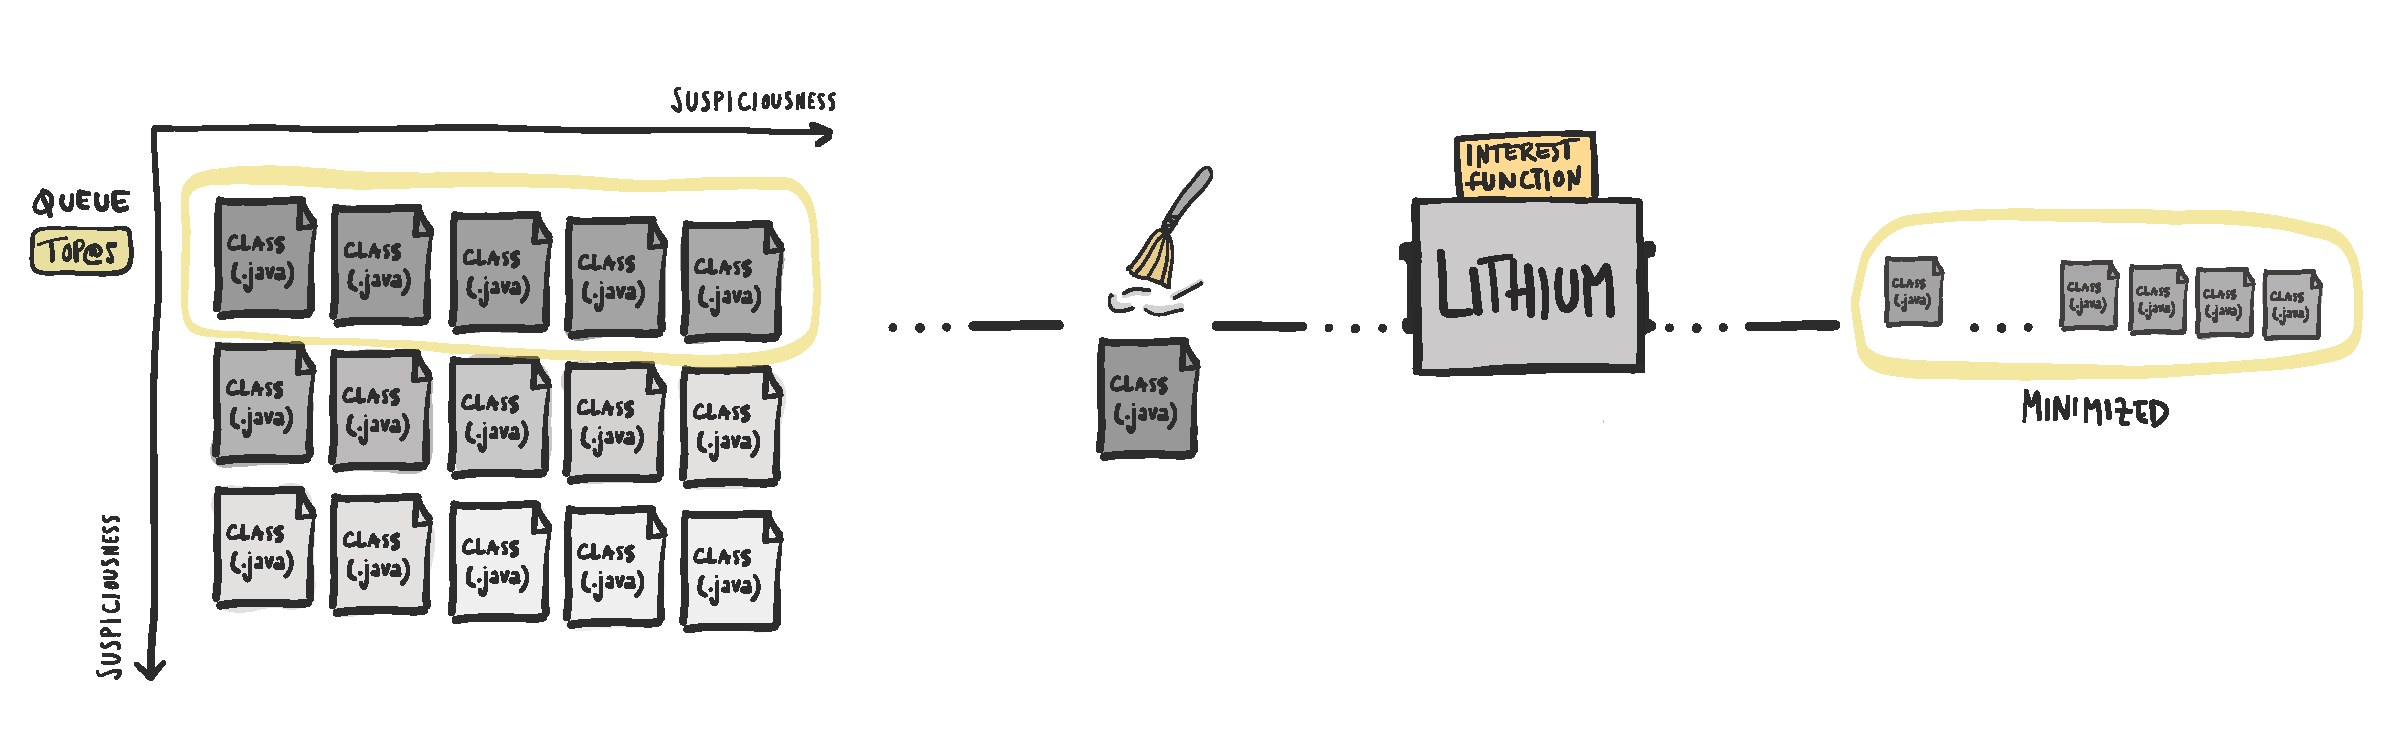
\includegraphics[width=1.0\textwidth]{figures/lithium.pdf}
% 	\caption{Simple illustration of the process to obtain the top-5 minimized classes from a project carrying a bug}
% \end{figure*}
%

%---------------------------------------------------------
%% \subsubsection{\label{sec:oracleheuristics}Oracle Heuristics.}~


%% The \cs{} technique is somewhat based on the \textit{statement deletion} mutant
%% operator of the mutation-based testing methodology. This operator was designed
%% based on the idea that each statement has an effect on the program output (i.e.,
%% oracle). Thus, testers are encouraged to design test sets that cause all
%% statements to be executed and generate outputs that are different from the
%% program under test.

%% Mozilla's Lithium takes as input a function of interest that can be designed
%% according to the problem to be solved. The function of interest determines if
%% the test case output is interesting or not. Our function simply compares the
%% failing test output with the output obtained when re-running again the failing
%% test after deleting the slice, as explained in Section~\ref{sec:slicing}. Thus,
%% if the initial test output is the same as the one after removing the slice
%% \{$c_2$,$c_5$\}, then the slice is removed. This means that the slice is not
%% necessary to reveal the fault because if removed the test output is still the
%% same. The output is extracted from the stacktrace obtained through the failing
%% test execution. The stacktrace provides information not only about the place
%% where the fault was revelead but also the path taken to get there. Thus, our
%% approach considers not only the exception caught by the failing test but also
%% the path that was taken to reveal the fault. The following provides an example:

%% \vspace{3mm}
%% \begin{myframe} \label{box:1}
%% junit.framework.AssertionFailedError, \\
%% at junit.framework.Assert.fail(Assert.java:55), \\
%% at junit.framework.Assert.assertTrue(Assert.java:22), \\
%% at junit.framework.Assert.assertFalse(Assert.java:39), \\
%% at junit.framework.Assert.assertFalse(Assert.java:47), \\
%% at junit.framework.TestCase.assertFalse(TestCase.java:219), \\
%% at org.jfree.chart.util.junit.ShapeUtilitiesTests.\\testEqualGeneralPaths(ShapeUtilitiesTests.java:212), \\
%% ...
%% \end{myframe}

%% Considering some of the stacktrace information about the path taken to reveal
%% the fault solved the issue of generic oracles (e.g., NPE or generic
%% AssertionFailedError expections as the one presented before) mentioned in
%% Theorem~\ref{the:1}. There are faults whose outputs could slightly differ from
%% one execution to another. For example, exceptions including information of
%% memory addresses. For these cases, it was developed a mechanism to compare the
%% rest of the output ignoring the identifier of the memory address. This heuristic
%% also handles StackOverflow oracles.
%---------------------------------------------------------

\section{Spectrum-based Fault Localization (\sfl)}
\label{sec:sfl}

\begin{wrapfigure}[8]{1}{0.25\textwidth}
  \hspace{-2ex}
  \centering
  \scriptsize
  \setlength{\tabcolsep}{3.5pt}
  \begin{tabular}{c|cccc|c}
    $\mathcal{T}$ & $c_1$    & $c_2$    & $\cdots$ & $c_M$    & $e$    \\ \hline
    $t_1$         & $\A{11}$ & $\A{12}$ & $\cdots$ & $\A{1M}$ & $e_1$  \\
    $t_2$         & $\A{21}$ & $\A{22}$ & $\cdots$ & $\A{2M}$ & $e_2$  \\
    \vdots        & \vdots   & \vdots   & $\ddots$ & \vdots   & \vdots \\
    $t_N$         & $\A{N1}$ & $\A{N2}$ & $\cdots$ & $\A{NM}$ & $e_N$  \\
  \end{tabular}
  \caption{An example spectrum.}
  \label{fig:spectrum-example}
\end{wrapfigure}

Spectrum-based fault localization is a statistical fault
localization technique that takes as input a test suite including at
least one failing test and reports on output a ranked list of
components likely to be in
fault~\cite{7390282,DBLP:conf/kbse/JonesH05,DBLP:journals/smr/LuciaLJTB14,DBLP:journals/jss/AbreuZGG09}. The
following are given in \sfl{}: a finite set $\mathcal{C}=\set{c_1,c_2,...,c_M}$
of $M$ system \emph{components}\footnote{A
component can be any code artifact of arbitrary granularity
such as a class, a method, or a statement~\cite{DBLP:journals/stvr/HarroldRSWY00}.};
a finite set $\mathcal{T} = \set{t_1,t_2,...,t_N}$ of $N$ system transactions,
which correspond to records of a system execution, such as test cases;
the error vector $e = \set{e_1,e_2,...,e_N}$, where $e_i = 1$ if
transaction $t_i$ has failed and $e_i = 0$ otherwise; and an
$N\times{}M$ coverage matrix $\mathcal{A}$, where $\A{ij}$ denotes the
coverage of component $c_j$ in transaction $t_i$.  The pair
$(\mathcal{A},e)$ is commonly referred to as
spectrum~\cite{DBLP:journals/stvr/HarroldRSWY00}. Figure~\ref{fig:spectrum-example}
shows an example spectrum.

Several types of spectra exist.  The most commonly used is called
hit-spectrum, where the coverage matrix is encoded in terms of binary
\emph{hit} (1) and \emph{not hit} (0) flags, \ie{}, $\A{ij} = 1$ if
$t_i$ covers $c_j$ and $\A{ij} = 0$ otherwise.  \sfl{} takes as input
the pair $(\mathcal{A},e)$ and produces on output a list of components
ranked by their faulty suspiciousness. To that end, the first step of
the technique consists of determining what columns of the matrix $A$
resemble the error vector $e$ the most.  For that, an intermediate
component frequency aggregator $n_{pq}(j)$ is computed $n_{pq}(j) =
|\{i\mid \A{ij}=p \wedge e_i=q\}|$. $n_{pq}(j)$ denotes the number of
runs in which the component $j$ has been active during execution ($p =
1$) or not ($p=0$), and in which the runs failed ($q = 1$) or passed
($q = 0$).  For instance, $n_{11}(j)$ counts the number of times
component $j$ has been involved ($p = 1$) in failing executions ($q =
1$), whereas $n_{10}(j)$ counts the number of times component $j$ has
been involved in passing executions. We then calculate similarity to
the error vector by means of applying \emph{fault predictors} to each
component to produce a score quantifying how likely it is to be
faulty.  Components are then ranked according to such likelihood
scores and reported to the user. Ochiai is one of those fault
predictors that has shown to perform
well~\cite{7390282,Pearson:2017:EIF:3097368.3097441}. The Ochiai
formula is given by the following equation
$\textit{ochiai}\,$=$\,\N{11}/\sqrt{(\N{11}+\N{01}) * (\N{11}+\N{10})}$.

\section{The \comb{} Approach}
\label{sec:approach}
\label{sec:comb}

This section describes \combpar{}, a technique where \ds{} and \sfl{}
work in tandem to solve the fault localization problem. To illustrate
the idea behind \combpar{}, consider a debugging scenario with five
components $c_{1..5}$ and five transactions $t_{1..5}$, two of which
are failing. Consider, additionally, that the component $c_2$ is
faulty.  Figure~\ref{fig:illustration} shows, at the left-hand side of
the arrow ($\Rightarrow$), an hypothetical spectra and its
corresponding ranking, produced with the Ochiai predictor. Each line
in the ranking shows, respectively, the rank/position, the component
label, and the Ochiai score (in parentheses).

We illustrate the workflow of the \comb{} approach for this scenario
in the following. Let us analyze components at the granularity of
statements.  First, \comb{} picks the first two statements at the top
of the ranking, $c_4$ and $c_3$, for further analysis.  (The cutoff
point is user-defined.) Second, the technique picks a failing test to
slice the code, say $t_2$. A slice is a set of statements. Let us
assume that the slice obtained for the transaction $t_2$ is $\{c_2,
c_5\}$, \ie, it excludes statements $c_4$ and $c_3$ that were
previously covered by the test. Finally, the spectra and ranking are
updated. The right-side of Figure~\ref{fig:illustration} shows the
modified spectra and ranking after slicing the code against $t_2$. It
is worth noting that the technique slices the code for every failing
tests. Intuitively, slicing enables the identification of statements
in the spectra whose values can be set to zero, \ie{}, the components
marked with $0$ are irrelevant to determine the test output.

Let us now observe the effect of this spectra modification on the
ranking. Analyzing the Ochiai formula, one observes that, for the
components $j$, which are not part of the slice of a failing test, the
combination reduces the value of $\N{11}$ and increases the value of
$\N{01}$. Therefore, suspiciousness of those components
decrease. Similar argument applies to other fault predictors. In the
running example from Figure~\ref{fig:illustration}, the components
$c_3$ and $c_4$, which are not in the slice of $t_2$, have their
suspiciousness reduced, enabling the faulty component $c_2$ to rise
from the third to the first position in the ranking.

\vspace{1ex}
To sum, the workflow of \comb{} consists of four steps:
\begin{enumerate}
  \itemsep0em
  \item\label{step:spectra} Compute spectra $S$ and ranking $R$ for
  the input test suite;
  \item\label{step:susp-files} Select top $k$ most suspicious classes, according to $R$;
  \item\label{step:compute-slice} Compute slicer for every suspicious
    file, obtained in Step~\ref{step:susp-files}, and every failing test;
  \item\label{step:group} Assemble all the resulting slicers of each failing test;
  \item Adjust spectra $S$, from step~\ref{step:spectra}, with
    the slices of each failing test, from
    step~\ref{step:group}, and then
	recompute the ranking.
\end{enumerate}

\begin{theorem}
  The rank of faulty statements cannot decrease if the slice includes
  the faulty statements.
\end{theorem}

The proof is based on the outlined argument that irrelevant
components $j$ have their ranks reduced as $\N{11}$ decreases and
$\N{01}$ increases. If those irrelevant components appear at positions
above the faulty component, it is possible that the faulty component
becomes more suspicious relative to $j$, \ie{}, the ranking of the
faulty component increases. If those components appear at positions
below the faulty components, the ranking of the faulty components is
unaffected.\hfill{\tiny$\blacksquare$}

\begin{figure}[t!]

  \centering
  \begin{subfigure}{0.5\textwidth}
    {\def\arraystretch{0.9}\setlength{\tabcolsep}{3pt}
      \begin{tabular}{c|ccccc|c}
        $\mathcal{T}$ & $c_1$    & $c_2$   & $c_3$ & $c_4$ &  $c_5$   & $e$    \\ \hline
        $t_1$         & 1 & 0 & 1 & 1 & 0 &\cmark  \\
        $t_2$         & 0 & 1 & 1 & 1 & 1 &\xmark  \\
        $t_3$         & 1 & 0 & 1 & 0 & 0 &\xmark  \\
        $t_4$         & 0 & 1 & 0 & 0 & 1 &\cmark  \\
        $t_5$         & 1 & 0 & 0 & 1 & 1 &\cmark \\
        \hline
      \end{tabular}
      \quad
      $\Rightarrow$
      \quad
      \begin{tabular}{c|ccccc|c}
        $\mathcal{T}$ & $c_1$    & $c_2$   & $c_3$ & $c_4$ &  $c_5$   & $e$    \\ \hline
        $t_1$         & 1 & 0 & 1 & 1 & 0 &\cmark  \\
        $t_2$         & 0 & 1 & {\cellcolor{Gray} 0} & {\cellcolor{Gray} 0} & 1 &\xmark  \\
        $t_3$         & 1 & 0 & 1 & 0 & 0 &\xmark  \\
        $t_4$         & 0 & 1 & 0 & 0 & 1 &\cmark  \\
        $t_5$         & 1 & 0 & 0 & 1 & 1 &\cmark  \\
        \hline
      \end{tabular}
    }
    \caption{Spectra update.}
    \label{fig:ds-reduction}
  \end{subfigure}

  \vspace{2ex}

  \begin{subfigure}{0.5\textwidth}
    \centering
    \begin{tabular}{cccccc}
      {\cellcolor{Gray}1} & {\cellcolor{Gray}$c_4$ (0.59)} & & 1 & $c_2$ (0.35) \\
      {\cellcolor{Gray}2} & {\cellcolor{Gray}$c_3$ (0.55)} & & 2.5 & $c_1$ (0.32)\\
      3 & $c_2$ (0.35) & \hspace{1ex}$\Rightarrow$\hspace{1ex} & 2.5 & $c_5$ (0.32)\\
      4.5 & $c_1$ (0.32) & & {\cellcolor{Gray}4} & {\cellcolor{Gray}$c_3$ (0.29)}\\
      4.5 & $c_5$ (0.32) & & {\cellcolor{Gray}5} & {\cellcolor{Gray}$c_4$ (0.00)}\\
    \end{tabular}
    \caption{Ranking update.}
  \end{subfigure}

  \caption{Modifications on spectra and ranking as result of slicing
    code against test $t_2$. Double arrow ($\Rightarrow$) indicates
    before and after.}
  \label{fig:illustration}
  \vspace{-2ex}
\end{figure}

%
\section{Evaluation}
\label{sec:eval}

We studied the following research questions:

%% The goal of this paper is to reassess whether the \comb{} approach yields
%% promising results under a more rigorous experimental methodology and a larger
%% dataset.\comments{The D4J dataset is about twice as large than the biggest test
%% suite used in previous studies.}

\newcommand{\rqone}{How effective is DS in eliminating code?}
\newcommand{\rqtwo}{How often does DS miss faulty statements?}
\newcommand{\rqthree}{How effective is \comb{} for bug localization?}

\begin{itemize}[leftmargin=0em]
\item[]{\textbf{RQ1.}}~\textit{\rqone{}}
\item[]{\textbf{RQ2.}}~\textit{\rqtwo{}}
\item[]{\textbf{RQ3.}}~\textit{\rqthree{}}
\end{itemize}

The first question evaluates the ability of dynamic slicing to reduce
the size of application code. Improvements on fault localization
depend on that ability. The second question addresses the problem that
affects all dynamic slicing
techniques~\cite{Lin:2018:BDE:3238147.3238163}---that of missing
faulty statements (see Theorem~\ref{the:1}). Developers would
not be able to successfully debug code for the cases that issue is
manifested. The third research question evaluates the impact of the
combination, as substantiated by \comb, to fault localization.

%%  shows that CS can
%% miss faulty statements because of imprecise oracles that guide the
%% slicing process.
%% Different slicers can miss faulty statements for different
%% reasons. In this paper, we used Critical
%% Slicing~\cite{DeMillo:1996:CSS:229000.226310}, which, in principle,

%
%
\subsection{Objects of Analysis}\label{sec:analysis}


We used subject programs from the \dfj{}
benchmark~\cite{just-defects4j-issta2014} in our evaluation.
Table~\ref{tab:df4j} shows size, number of tests, and number of
faults, for each considered program.

\begin{table}[h]
  \small
  \centering
  \setlength{\tabcolsep}{4pt}
  \begin{tabular}{lrrr}
    \toprule
    Project            & Size (LOC) & \# Tests & \# Faults \\ %\comments{& Failing Test Cases &}
    \midrule
    \lang{}            & 111,751  & 6,057 & 65       \\   %\commentst{& 124   &  -}\\
    \cmath{}           & 306,276  & 26,797 & 104     \\   %\comments{& 177   &  -}\\
    %      \closure{}         & 149,521  & 27,930  & 133     \\   %\comments{& 350   &  -}\\
    \chart{}           & 230,159  & 8,458 & 26      \\  %\comments{& 92    &  -}\\
    \jtime{}           & 141,610  & 3,289 & 27       \\   %\comments{& 76    &  -}\\
    \mockito{}         & 22,787  & 8,835 & 38    \\     %\comments{& 118   &  -}\\
    \bottomrule
  \end{tabular}
  \caption {Characterization of \dfj{} subjects.}
  \label{tab:df4j}
\end{table}
\normalsize

\lang{} is a
library that provides a set of helper utilities for the
{\small\texttt{java.lang}} API. \cmath{} is a lightweight library of
self-contained mathematics and statistics components.\comments{ The
  \closure{} is a toolset for turning JavaScript files into smaller
  scripts for faster download and execution in the browser.} \chart{}
is a Java library for creating charts.  \jtime{} is a lightweight
library that aims to replace the default Java
{\small\texttt{java.util.Date}} classes providing simpler
APIs. \mockito{} is a mocking testing framework.

%% Originally, this benchmark includes six different subjects and 395
%% faults (Table \ref{tab:df4j}).

%%%%%%%%%%%%%%%%%%%%% I commented because there are just two cases;
%%%%%%%%%%%%%%%%%%%%% not much information added (that could not be
%%%%%%%%%%%%%%%%%%%%% said in text). -Marcelo
%% \begin{figure}[h]
%%   \vspace{-0.5cm}
%% 		\centering
%% 		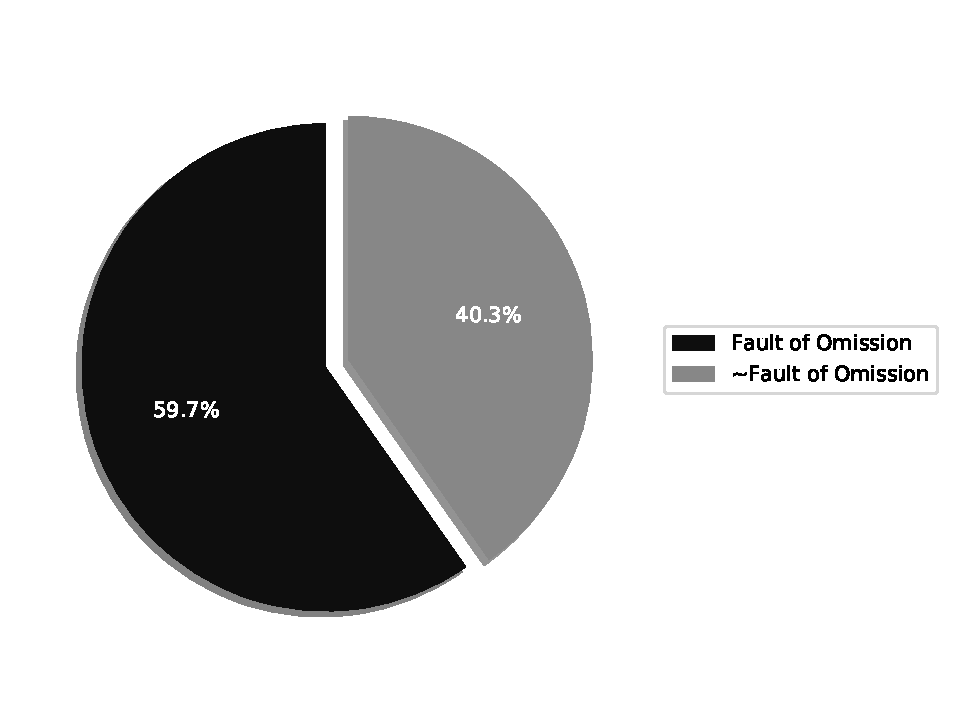
\includegraphics[width=0.42\textwidth]{figures/defects4j.pdf}
%% 		\vspace{-0.75cm}
%% 		\caption{Faults of omissions' distribution}
%% 		\label{fig:foos}
%% \end{figure}

As to quantify complexity of fault localization on this dataset, we
additionally counted the number of cases of ``fault of omission'', a
popular metric in fault localization research for that
purpose~\Fix{cite}. A fault of omission occurs when
\Fix{...explain...}. Intuitivelly, the ability of techniques to
produce good diagnosis in those cases reduce as \Fix{...explain...}. A
total of $59.7\%$ of the cases in this dataset manifest fault of
omission, which is a good indication of difficulty.

%in producing
%high-qualitiy diagnosis.

%\subsection{Experimental Methodology}
%\label{sec:methodology}

\subsection{Techniques}
One important independent variable for this study is the scope of
dynamic slicing. Slicing the entire code would be unacceptably
expensive as Critical Slicing needs to re-compile the affected file at
every iteration, \ie{}, after deleting statements and before checking
the oracle (see Section~\ref{sec:slicing}). We control the scope of
slicing through the variable $k$, which denotes the number of distinct
files that dynamic slicing will minimize. In this study, we used 5 and
10 as the values of $k$. The $k$ files for minimization are selected
from the \sfl{} ranking as follows. First, we build a rank of files by
determining, for each ranked statement, the file that declares
it. Then, we select the top $k$ distinct files from such file ranking.
\Rui{we should say that k follows from typical SFL metrics (top k)}

The techniques we evaluate in this study are \combpar{k} and
SFL$^{k}$, which is the comparison baseline. \combpar{k} is as defined
in Section~\ref{sec:approach} (see Step 2 of the workflow) whereas
SFL$^{k}$ is as SFL, but it produces a ranking including exclusively
the statements from the best-$k$ ranked files.

%% To evaluate the effectiveness of \comb{}, following related work, we compared
%% its performance with \sfl{} for each fault from the dataset, for $k\in\{5,10\}$,
%% where $k$ is the number of classes comprising the highest faulty statements.
%% These classes are obtained directly from the ranking which is calculated through
%% \sfl{}.



%% For each fault, spectra is updated and the fault ranking is
%% re-calculated but only considering the $k$ highest faulty classes. We refer to
%% these variations as SFL$^{k}$. After slicing each class of the top $k$ of the
%% highest faulty classes for each fault, the initial spectra is updated based on
%% the slicer output and the fault ranking is re-calculated. We refer to these
%% variations as \combpar{k}.

\subsection{Results}

This section answers the research questions.

%% proposed and discuss the
%% results obtained. Our approach was capable of slicing a total of $260$ faults
%% from $5$ different  projects.
%% \textbf{RQ1} evaluates how effective is \ds{} on reducing the test cases, \textbf{RQ2} reviews
%% one of the main issues of \ds{} - missing faulty statements - and
%% \textbf{RQ3} discusses how effective is the \combpar{k} approach against
%% \sfl{}$^{k}$.


\begin{table*}[t!]
	\small
	% \setlength{\tabcolsep}{3pt}
	\centering
	  \begin{tabular}{l|cccc|cccc|c}
		\toprule
		\multirow{2}{*}{Project}            & \multicolumn{4}{c|}{\sfl{}$^{k}$}  & \multicolumn{4}{c|}{\combpar{k}} & \multirow{2}{*}{\# Faults} \\

		            & \# $k = 5$ & \% $k = 5$ & \# $k = 10$ & \% $k = 10$
					& \# $k = 5$ & \% $k = 5$ & \# $k = 10$ & \% $k = 10$ &  \\
		\midrule
		 \lang{}         &  55 & 84.6\%  & 55  & 84.6\%
		 				& 65 & 100\% & 63 & 96.9\% & 65      \\
		\cmath{}           & 85 & 81.7\%  & 89 & 85.6\%
						& 93 & 89.4\% & 99 & 95.2\% & 104  \\   %\comments{& 177   &  -}\\
		% \closure{}         & 62.41 \%  & 72.18 \%  & 9.77 \%     \\   %\comments{& 350   &  -}\\
		\chart{}          & 22 & 84.6\% & 24 & 92.3\%
						& 20 & 76.9\% & 22 & 84.6\% & 26    \\
		\jtime{}          & 21 & 77.8 \% & 22 & 81.5 \%
				& 22 & 81.5\% & 23 & 85.2\% & 27     \\
		 \mockito{}      & 24  & 63.2\% & 27 & 71.1\%
		 				& 27 & 71.1\% & 30 & 78.9\% & 38 \\\midrule
	 Total      & 207  & 79.6\% & 217 & 83.5\%
	 				& 227 & 87.3\% & 237 & 91.2\% & 260 \\
		\bottomrule
	\end{tabular}
  \caption {Number of faults where at least one of the faulty-statements is in the \sfl{}$^{k}$ and \combpar{k} report}
  \label{table:fsws}
\end{table*}


%% This subsection aims to report the performance of the \ds{} technique
%% on slicing de faults of $5$ \dfj{} projects.


\subsubsection{\label{rq:1}RQ1: \textit{\rqone}}

A necessary but insufficient condition for improvement of fault
localization with \comb{} is that dynamic slicing eliminates a high
amount of code in the best ranked files. Table \ref{tab:red} shows, as
percentages, the average reduction on the sum of top file sizes
obtained with dynamic slicing for different values of
$k$.\Mar{$\leftarrow$sofia, please check.} Overall, results indicate
that dynamic slicing substantially reduces the size of highly-ranked
files. \Mar{sofia, it would be more convincing if you (additionally)
  show reduction wrt to the the parts of the file that are covered.}

%% obtained for each project after slicing the top $5$ and
%% $10$ of classes comprising the highest faulty statements. We observed
%% a reduction of $30.23\%$ in the projects considered in our study.

\begin{table}[H]
  \small
	\centering
	\setlength{\tabcolsep}{4pt}
	\begin{tabular}{lrr}
		\toprule
		Project             &  \multicolumn{1}{c}{$k=5$} & \multicolumn{1}{c}{$k=10$} \\ %\combpar{5}  & \combpar{10}
		\midrule

        \lang{}            & 1.40 & 31.46\\
        \cmath{}           & 10.30 & 12.34\\
        %\closure{}          &  & \\
		\chart{}			& 59.30 & 53.64 \\
        \jtime{}            & 17.27 & 32.02\\
        \mockito{}          & 16.54 & 21.67\\

		\bottomrule
	\end{tabular}
	\caption {\ds{} reduction, as percentages. Higher is better.}
	\label{tab:red}
\end{table}
\normalsize

\subsubsection{RQ2: \textit{\rqtwo}}
\label{rq:2}

\begin{table}[H]
  \small
	\centering
	\setlength{\tabcolsep}{4pt}
	\begin{tabular}{lrr}
		\toprule
		Project             &  \multicolumn{1}{c}{$k=5$} & \multicolumn{1}{c}{$k=10$} \\ %\combpar{5}  & \combpar{10}
		\midrule

        \lang{}            & 100 & 96.9\\
        \cmath{}           & 89.4 & 95.2\\
        %\closure{}          &  & \\
		\chart{}			& 76.9 & 84.6 \\
        \jtime{}            & 81.5 & 85.2\\
        \mockito{}          & 71.1 & 78.9\\

		\bottomrule
	\end{tabular}
	\caption {\ds{} performance on capturing faulty statements, as percentages.}
	\label{tab:red}
\end{table}
\normalsize

%% For automated debugging that
%% means that it will not be in the diagnostic report and therefore has a negative
%% impact in the fault localization accuracy. 


%% In \textbf{RQ2}, our concern is to evaluate how often \ds{} misses faulty
%% statements, since it is one of the main issues of dynamic slicing techniques. This
%% is particularly important because when \ds{} misses a faulty statement

%% of both techniques, \sfl{}$^{k}$ and \combpar{k}

A fundamental issue of purely dynamic slicing techniques, critical
slicing in particular, is the risk of discarding faulty statements
(see Section~\ref{sec:slicing}). This research question evaluates the
practical impact of this conceptual issue. Table~\ref{table:fsws}
presents the number of faults where at least one of the faulty
statements appears in the final reports.\Mar{$\leftarrow$this seems a
  sensible choice that needs reasonable (to-the-point)
  justification. is there a rationale for this?  if not, was this
  choice used in other study? if yes, just say it was used and cite.}
More precisely, we look for faulty statements in the top 5 and 10 most
suspicious classes (as per the file ranking).

\Mar{CRITICAL: Sofia, I am really confused here. Is there a reason for
  why you chose not to show the proportion of cases where **DS** (not
  SFL(k) or \combpar{k}) includes the faulty statement? Wouldn't it be
  sufficient and simpler/clearer answering this question in terms of
  DS for k=5,10? (Note that the question is about DS.) On a similar
  note, considering this metric, I don't understand how SFL(k) can
  produce different result compared to \combpar{k}. I thought the
  difference in this case would only be the position in the
  ranking. This is counter-intuitive and needs a good explanation.}
Table~\ref{table:fsws} compares \sfl{}$^{k}$ and \combpar{k} with
respect to the metric number of cases where a faulty statement appears
in the ranking. Results show that \combpar{k} finds the faulty
statements \Fix{faster}\Mar{faster? chose another word.} than
\sfl{}$^{k}$.\Mar{I will revise the rest of this par. when I
  understand what is going on here...}  \sfl{}$^{5}$ finds $207$
($79.6\%$) faults whereas \combpar{5} finds $227$ ($87.3\%$) faults
for $k=5$, i.e., \combpar{5} misses $20$ ($7.7\%$) less faults
compared to \sfl{}$^{5}$. \sfl{}$^{10}$ finds $217$ ($83.5\%$) faults
whereas \combpar{10} finds $237$ ($91.2\%$) for $k=10$, i.e.,
\combpar{10} misses less $20$ ($7.7\%$) faults than
\sfl{}$^{10}$. There is also a significant difference within each
technique. Generally, the majority of faulty statements are found on
the $5$ highest ranked faulty classes. There are few cases where the
faulty statements are only found if the approach considers the first
$10$ highest ranked faulty classes \combpar{10} is the variant of our
approach that performs better \textbf{missing only 23 out of 260
  (8.8\%) cases}.

\subsubsection{RQ3: \textit{\rqthree}}

In \textbf{RQ3}, we evaluate the effective impact of combining \ds{}
with \sfl{} to improve fault localization.

The first experiment we ran to assess impact consisted of measuring
the \emph{difference of diagnosis cost}. This metric has been
previously used in other studies~\Fix{cite cite}. More specifically,
we computed $\Delta{}C = C(\textrm{SFL$^{k}$}) -
C(\textrm{\combpar{k}})$, where $C$ denotes the diagnosis cost and is
obtained by computing the mean position in the ranking of all buggy
statements. $\Delta C >0$ means that the position of the faulty
statement has decreased with \combpar{k}, \ie{}, the combination had a
positive impact. $\Delta C <0$ means that \combpar{k} performs worse
compared to its baseline. That could happen if dynamic slicing misses
the faulty statement---the statements not included in the slice will
have their suspiciousness scores reduced and ranks potentially
reduced. $\Delta C=0$ means that the faulty statement remained in the
same position.  It is worth noting that we assume a perfect bug
understanding, i.e., if the developer sees the bug in the ranking, he
is able to precisely determine if it is the faulty one.

\Mar{I see there are different results/metrics/tables. We need to
  organize this better, with sub-questions or stating different
  other experiments to answer the main question.}


\Mar{---------------------- I am here}

Figure \ref{fig:diagnosis} reports the cost of diagnosis of using \combpar{5} and \combpar{10} instead of \sfl{}$^{5}$ and \sfl{}$^{10}$,
respectively. For $k=5$, we observe that in $30$ ($11.5\%$) of the faults
the position of faulty statements decreases
in the ranking, $97$($37.3\%$) of the faults the position of faulty statements increases in the rankinh whereas $133$ ($51.2\%$) of the faults the position of faulty stamenets remains the same. For $k=10$, we observe an increasing of $20$ cases where the position of faulty statements increases in the ranking $117$ ($45.0\%$).
The number of cases whose faulty statements position remained the same are $110$ ($42.3\%$) and that suffered a decrease in the ranking is $33$ ($12.7\%$).

Table~\ref{table:st}, reports the average rank of all faulty
statements of the \dfj{} faults considered to the study after applying both
techniques, \sfl{}$^{k}$ and \combpar{k} for $k=5$ and $k=10$. $33$ of the $260$
faulty versions are cases whose faulty statements decreased in the ranking list due to being a fault of omission case or due to limitations regarding the test design which \ds{} could not handle. Thus, we report both values in Table~\ref{table:st}. In bold, we present the
results of the $227$ faults that do not contain the cases that are result of the limitations mentioned before. Inside parentheses, we present the
rank results for all faults. The \combpar{k} combination yields an improvement
of $17.3$ on the rank mean of the dataset faulty statements when using $k=5$.
Instead, if $k=10$ is considered the proposed approach returns an improvement of
$6.1$ on the rank mean of all faulty statements.
This $227$ faults contain cases where the faulty class was not in the choosen set of classes $k$ and a high amount of cases where the improvement was none. Yet,
if we only consider the faults ($116$) where there was improvement in at least
one of the variants ($k=5$ or $k=10$) the \textbf{ranking increases in a mean of 41.1} for
$k=5$ and \textbf{18.7} for $k=10$. The maximum improvement obtained in the \sfl{} rank was  $3170.5$ for $k=5$ and $209$ for $k=10$, which is significant.


Although this dataset has more than $50\%$ of fault of omissions,
our simple slicing approach was capable of improving the ranking of $95$ faults for
$k=5$ and $115$ faults for $k=10$. Table \ref{table:st} presents the statistics
to determine if the observed results are statistically significant. Shapiro-Wilk
tests the null hypothesis that results are drawn from a normal distribution. The
test is perfomed for all techniques and its variants. With $99\%$ of confidence,
the results tell us that the distributions are not normal. Given that $C$ is not
normally distributed, we use the non-parametrical statistical hypothesis test
Friedman. The null-hypothesis is that the ranking results of all techniques and
variants are the same. With $99\%$ of confidence, the results show that the
distributions are distinct. To understand which techniques perform differently 
- i.e., \textit{Does \combpar{10} perform differently than \sfl{}$^{10}$} -
we performed a Siegel post-hoc analysis. Figure
\ref{fig:performance} reports the results of Siegel analysis for all pairs of techniques. Each square represents the significance between the correspondent techniques, i.e., if it is significant it means that the techniques perform differently. With $95\%$ of confidence, it is possible to confirm that the performance of all techniques is different expect when comparing \combpar{5} with \combpar{10}.

It is worth noting that Automated
Program Repair techniques may directly benefit from this study to improve their
results.

\Rui{Weakness: there has to be discussion on whether there is potential/promising
results somewhere.}

\begin{figure}[h]
		\centering
		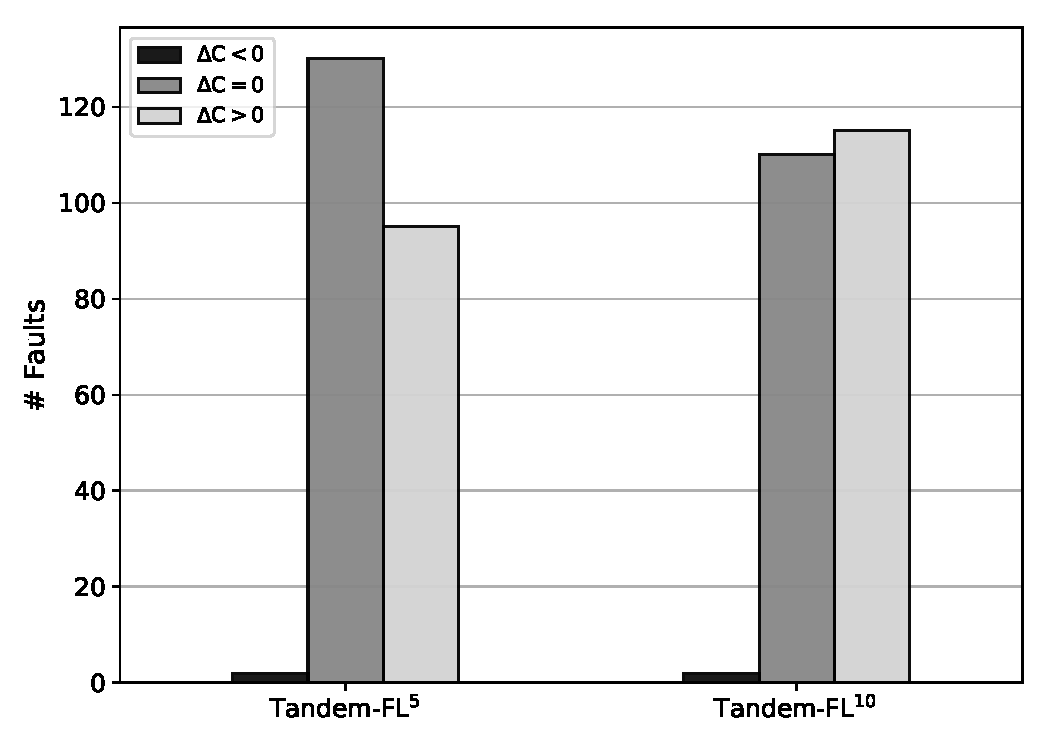
\includegraphics[width=0.42\textwidth]{figures/performance.pdf}
		\caption{Cost of diagnosis of using \combpar{5} and \combpar{10} instead of \sfl{}$^{5}$ and \sfl{}$^{10}$, respectively}
		\label{fig:diagnosis}
\end{figure}

\begin{table}[h]
	\tiny
	\centering
	\setlength{\tabcolsep}{3pt}
	\begin{tabular}{@{}c|c|c|c|c@{}}
\toprule
  & SFL$^{5}$      & SFL$^{10}$     & \combpar{5}              & \combpar{10}              \\ \midrule
Mean & \textbf{590.7} (584.3)   &  \textbf{512.7} (516.4)  & \textbf{573.4} (679.7)  & \textbf{506.6} (614.0)   \\ \midrule
Median & \textbf{46.5} (49.4)    & \textbf{54.5} (53.0) & \textbf{42.7} (69.3)  & \textbf{40.0} (56.9)\\ \midrule
Variance & \textbf{1257.0} (1223.1)  &  \textbf{1171.5} (1148.1) & \textbf{1239.1} (1352.4) &  \textbf{1167.0} (1294.9) \\ \midrule
Shapiro-Wilk &\makecell{$W$ = 0.52 \\ $p$ = 1.75 x $10^{-24}$} & \makecell{$W$ = 0.48 \\ $p$ = 2.50 x $10^{-25}$} & \makecell{$W$ = 0.51 \\ $p$ = 1.10 x $10^{-24}$} & \makecell{$W$ = 0.48 \\ $p$ = 2.26 x $10^{-25}$}  \\ \midrule
Friedman & \multicolumn{4}{c}{\makecell{$\chi^{2}$ = 162.61 \\ p-value = 5.00 x $10^{-35}$}} \\
\bottomrule
\end{tabular}
  \caption {Statistical tests}
  \label{table:st}
\end{table}

\begin{figure}[h]
	\vspace{-1.2cm}
		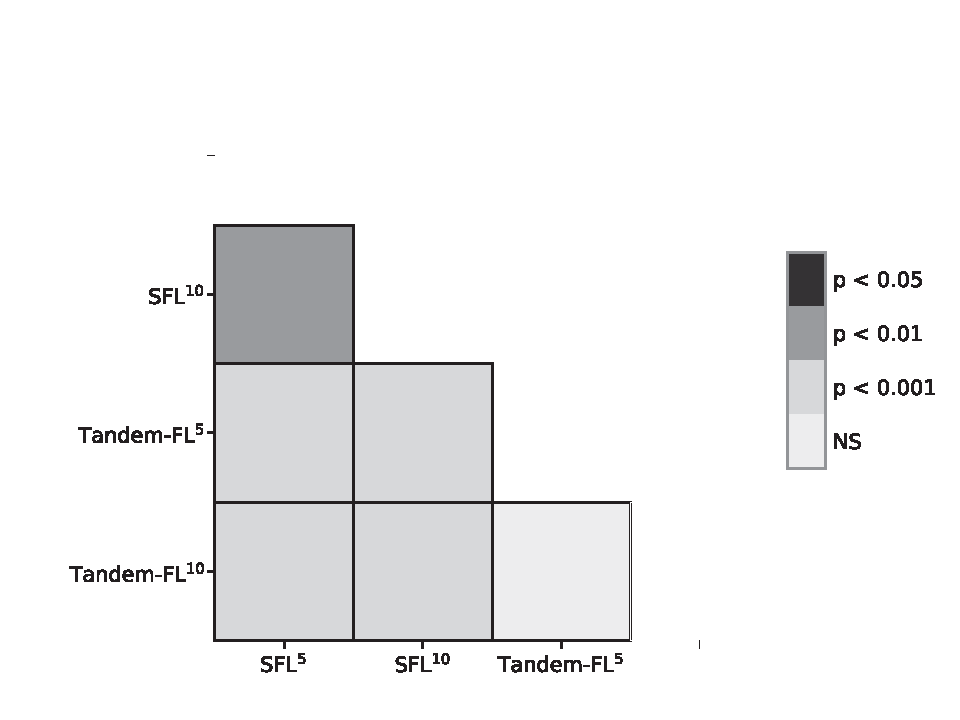
\includegraphics[width=0.45\textwidth]{figures/heatmap_nemenyi_result.pdf}
		\caption{Siegel post-hoc analysis results}
		\label{fig:performance}
\end{figure}

\subsection{Threats to validity}

\Mar{incorporate this here. we were presenting this too early (initial
  par. of results). not very appealing ;)}
\Fix{
The remaining faults were not considered because
(1) faults belong to the \closure{} project which requires high CPU to perform
the \combpar{k} evaluation  or (2) faults whose test outputs were not
reproducible in the machine used to run the experiments.
}

%
A potential threat to external validity related to the set of programs used in
our study. When choosing the projects for our study, our aim was to opt for
projects that resemble a general and large-sized application. To reduce
selection bias and facilitate the comparison of our results, we decided to
choose a benchmark that is popular in the community~\cite{just-defects4j-issta2014}.

A potential threat to construct validity relates to the choice of oracle generation
for the Lithium toolset. However, we argue that our choice is able to capture whether
a program is failing because of the same reason.

The main threat to internal validity lies in the complexity of several of the tools
used in our experiments, most notably the Lithium toolset, the SFL diagnosis tool,
and the implementation of \comb{}.
%
\section{Related Work}
\Rui{Introductory sentences should say something like: model-based software
debugging, from the DX community, has been shown to be similar to slicing
Mayer and Stumptner, 2008; Wotawa and Nica; etc. Having said that, not many
interesting techniques having been pursued because of scalability. We have
achieved it with a type of program slicing --- critical slicing. Next, we
visit the previous works on program slicing and SFL, without the idea of
being exhaustive, but merely discussing the works that we deem relevant for
this paper.}

\Rui{revisit sentences; check if recent papers are cited.}

\subsection{Program Slicing}

Program Slicing is an old technique with several applications in PL
and SE research~\cite{Weiser:1981:PS:800078.802557}. Slicing can be
implemented in different ways. Dynamic Slicing has found its main
application in fault
localization~\cite{Agrawal:1990:DPS:93542.93576}---in this application
context, failing tests exist. Research in this area has mainly focused
on slicing code
efficiently~\cite{Wang:2008:DSJ:1330017.1330021,Wang:2004:UCB:998675.999455}
and avoiding data and control omission
errors~\cite{Zhang:2007:TLE:1250734.1250782,Lin:2018:BDE:3238147.3238163}. Omission errors correspond to the
cases where tests fail because some part of the code was not executed
when it should. Dynamic fault localization techniques cannot hope to
soundly report bugs in those cases. The issue is that incorporating
static information to capture those cases can result in unacceptably
large slices, which defeats the purpose of reducing the fault search
space. It is worth noting that, conceptually, the \sfl{}+\ds{} combination
can be used with any form of dynamic slicing. We chose an
implementation of Critical
Slicing~\cite{DeMillo:1996:CSS:229000.226310} for its generality.


\subsection{SFL}

Statistics-based techniques (e.g., ~\cite{Pearson:2017:EIF:3097368.3097441}) are
popular automated fault localization techniques within the Software Engineering
community. They correlate information about program fragments that have been
exercised in multiple program execution traces (also called \textit{program
spectra}) with information about successful and failing executions. By doing
that, statistics-based approaches yield a list of suspect program fragments
sorted by their likelihood to be at fault. Since this technique is efficient in
practice, it is attractive for large modern software systems ~\cite{Zoeteweij:2007:DES:1251988.1253298}.

Spectrum-based fault localization (\sfl{}) is amongst the most common statistical
fault localization technique that takes as input a test suite including at least
one failing test and reports on output a ranked list of components likely to be
in fault ~\cite{FLSurvey2016,DBLP:conf/kbse/JonesH05,DBLP:journals/smr/LuciaLJTB14,DBLP:journals/jss/AbreuZGG09}.

\subsection{Combination of \sfl{} and Slicing}

Prior work has investigated the combination of dynamic slicing and
spectrum-based fault
localization ~\cite{Wotawa:2010:FLB:1848650.1849235,Alves:2011:FUD:2190078.2190115,DBLP:conf/ecai/HoferW12,lei-mao-dai-wang-2012,slicing-sfl-repair}. Although
the methodology used in these papers vary, the overall message is that
the combination is valuable. Note that slicing alone does not provide
the guarantee of improvement to \sfl{} as statements discarded with
slicing could have been ranked lower compared to faulty
statements. This paper differs from prior work in that it uses a much
larger dataset of programs and faults and a more rigorous experimental
methodology.
%
\section{Conclusions and Future Work}
\label{sec:conc}
%

\Fix{
The main lesson of this work is that
fault localization research should consider compare new techniques
against this combination.}

Several approaches have been proposed in the literature to improve debugging
costs through automated software fault diagnosis to reduce time-to-market,
while maintaining high quality standards. In this domain, Dynamic Slicing (DS)
and Spectrum-based Fault Localization (SFL) are very popular fault diagnosis t
echniques and normally seen as complementary. This paper reports the outcome of
a study using real-world applications with the goal of demystifying the impact
of combining DS with SFL. The results of our empirical study show that, in
practice, DS rarely misses faulty statements (23 misses in 260 cases) and that
the DS-SFL combination improves the diagnostic accuracy in 51\% of the faults.
Hence, we found that, despite tacit opinions of the research community about
the usefulness of DS in automated debugging, we found the combination practical
and effective, and encourage new SFL techniques to be evaluated against that
optimization.

Future work is as follows: bla bla.

%
%\section*{Acknowledgments}
%include only after review.
{
  \small
  \balance
  \bibliographystyle{named}
  \bibliography{paper}
}

\end{document}
